\documentclass[a4paper,12pt]{article} 
\usepackage{geometry}
\geometry{
	a4paper,
	total={170mm,257mm},
	left=20mm,
	top=20mm,
}
\usepackage{titlesec}
\titlelabel{\thetitle.\quad} %точка в section

%%% Работа с русским языком
\usepackage{cmap}                           % поиск в PDF
\usepackage{mathtext} 			 	       % русские буквы в формулах
\usepackage[T2A]{fontenc}               % кодировка
\usepackage[utf8]{inputenc}              % кодировка исходного текста
\usepackage[english,russian]{babel}  % локализация и переносы

%Математика
\usepackage{amsmath,amsfonts,amssymb,amsthm,mathtools} % AMS
\usepackage{icomma} % "Умная" запятая

%% Шрифты
\usepackage{euscript}	 % Шрифт Евклид
\usepackage{mathrsfs} % Красивый матшрифт

%% Команды
\DeclareMathOperator{\const}{\mathop{const}}

%% Перенос знаков в формулах
%\newcommand*{\hm}[1]{#1\nobreak\discretionary{}
%	{\hbox{$\mathsurround=0pt #1$}}{}}
\usepackage[pdftex]{graphicx}

%%% Заголовок
\author{Хохлов Андрей, Коротков Антон}
\title{Практическая работа 6 \\
	\textbf{Химические свойства галогенов и их соединений}}
\date{28 марта 2024}

\begin{document}
	
	{\Large \maketitle}
\section{Получение хлора и хлорной воды (демонстрационно на группу)}	
В круглодонную колбу, снабженную капельной воронкой и газоотводной трубкой, поместили
немного кристаллического оксида марганца(IV). В капельную воронку налили раствор
концентрированной соляной кислоты и по каплям прилили ее к оксиду марганца(IV) при
нагревании. 
\begin{figure}[h]

\centering

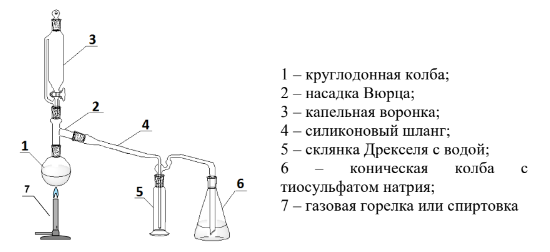
\includegraphics[scale=1.1]{1.png}

\caption{Установка для получения хлорной воды}

\label{fig:mpr}
\end{figure}
В круглодонной колбе в процессе ОВР образуется газообразный хлор. 
\begin{equation} 
\mathrm{MnO_2+4HCl \longrightarrow MnCl_2 + Cl_2\uparrow + 2H_2O } 
\end{equation}
Его пропустили через воду, находящуюся в склянке Дрекселя, наполовину заполненную водой.
При насыщении хлором холодной воды часть молекул $Cl_2$ диспропорционирует:
\begin{equation} 
\mathrm{Cl_2 + H_2O\leftrightarrows  HCl + HClO} 
\end{equation}
Но $\mathrm{HClO}$ постепенно разлагается на соляную кислоту и кислород, получаем хлорную воду.
\section{Окисление иона железа(II) хлором}
В две пробирки поместили по 1–2 микрошпателя сухой соли Мора. В первую пробирку
добавили 3–4 капли дистиллированной воды, во вторую – столько же капель хлорной воды.
Растворы разделили на две пробирки, в одну добавим роданид натрия, а в две другие пробирки добавим по каплям раствор аммиака, до
появления осадка в пробирках. 

В первой пробирке выпал гидроксид железа(II), осадок зелёного цвета.
\begin{equation} 
\mathrm{Fe(NH_4)_2(SO_4)_2 + NH_3 + H_2O \longrightarrow Fe(OH)_2\downarrow + (NH_4)_2SO_4} 
\end{equation}

Во второй пробирке выпал коричневый гидроксид железа(III)
\begin{equation} 
\mathrm{Fe(NH_4)_2(SO_4)_2 + Cl_2+H_2O \longrightarrow Fe_2(SO_4)_3+(NH_4)_2SO_4+HCl} 
\end{equation}
\begin{equation} 
\mathrm{Fe_2(SO_4)_3 + NH_3 + H_2O \longrightarrow Fe(OH)_3\downarrow +(NH_4)_2SO_4} 
\end{equation}

\section{Получение бромной воды и иодной воды}
В пробирку положили 0,5 г твердого бромида калия, добавили к нему 1 мл 2М соляной
кислоты, а затем – осторожно, по каплям – раствор гипохлорита натрия. Раствор стал \textbf{соломенно-жёлтым}. Мы получили бромную воду
\begin{equation}
    2KBr + NaClO + 2HCl \longrightarrow Br_2 + NaCl + 2KCl+ H_2O
\end{equation}


Выполнили аналогичный опыт, заменив бромид калия иодидом калия. Раствор стал \textbf{бурым} 
\section{Сравнение окислительных свойств галогенов}
В три пробирки налили по 1 мл растворов: в первую – бромида калия, во вторую и третью –
иодида калия. Во все три пробирки добавили по 1 мл органического растворителя. В две пробирки
с растворами бромида и иодида калия добавили по 1 мл хлорной воды, в третью пробирку с
раствором иодида калия прилили 1 мл бромной воды. 

 
В первой пробирке слой гексана окрасился в соломенно-жёлтый. Был \textbf{экстрагирован бром}
\begin{equation} 
\mathrm{2KBr+ Cl_2  \longrightarrow 2KCl + Br_2} 
\end{equation}


 
Во второй пробирке слой гексана окрасился в лиловый. Был \textbf{экстрагирован йод}
\begin{equation} 
\mathrm{2KI+ Cl_2  \longrightarrow 2KCl + I_2} 
\end{equation}


В третьей пробирке слой гексана окрасился в лиловый. Был \textbf{экстрагирован йод}
\begin{equation} 
\mathrm{2KI+ Br_2  \longrightarrow 2KBr + I_2} 
\end{equation}
В четвертую пробирку внесли 0,5 мл йодной воды и добавили к ней 1,5 мл хлорной воды.


В ней всё обесцветилось.
\begin{equation} 
\mathrm{5Cl_2 + I_2 + 6H_2O \longrightarrow 10HCl + 2HIO_3} 
\end{equation}
Йод - хороший восстановитель, ведь ему намного легче отдавать электроны, чем его более высоким собратьям по группе. 
\section{Восстановительная активность галогенид-ионов}
Поместили в одну пробирку несколько кристаллов бромида калия, а в другую – иодида калия.
В каждую пробирку добавили по 2–3 капли концентрированной серной кислоты. Началась бурная
реакция.

В первой пробирке слой гексана окрасился в соломенно-жёлтый. Сернистым газом потравило знатно. Был \textbf{экстрагирован бром}
\begin{equation} 
\mathrm{2KBr+ H_2SO_4  \longrightarrow 2KHSO_4 + SO_2\uparrow + Br_2 +2H_2O} 
\end{equation}

Во второй пробирке слой гексана окрасился в фиолетовый. Появился характерный запах тухлых яиц. Был \textbf{экстрагирован йод}
\begin{equation} 
\mathrm{8KI + 9H_2SO_4  \longrightarrow 8KHSO_4 +H_2S \uparrow + 4I_2 +4H_20}
\end{equation}

Из этих реакций можно понять, что йодводород - лучший восстановитель, чем бромо и хлороводороды.
\section{Качественные реакции на галогенид-ионы}
\subsection{C нитратом серебра}
а) В три пробирки поместили по 3–5 капель растворов солей: в первую пробирку – хлорида
натрия, во вторую – бромида калия, в третью – иодида калия. В каждую пробирку добавили 1–2
капли раствора нитрата серебра до выпадения характерных творожистых осадков галогенидов
серебра. 
В первой пробирке белый творожистый осадок
\begin{equation} 
\mathrm{NaCl + AgNO_3  \longrightarrow AgCl\downarrow + NaNO_3 } 
\end{equation}
Во второй пробирке желтоватый осадок
\begin{equation} 
\mathrm{KBr + AgNO_3  \longrightarrow AgBr\downarrow + KNO_3 } 
\end{equation}
В третьей пробирке жёлтый осадок
\begin{equation} 
\mathrm{KI + AgNO_3  \longrightarrow AgI\downarrow + KNO_3 } 
\end{equation}
\subsection{C нитратом свинца}
В первой пробирке малозаметный белый осадочек
\begin{equation} 
\mathrm{2NaCl + Pb(NO_3)_2  \longrightarrow PbCl_2\downarrow + 2NaNO_3 } 
\end{equation}
Во второй пробирке белый осадок
\begin{equation} 
\mathrm{2KBr + Pb(NO_3)_2  \longrightarrow PbBr_2\downarrow + 2KNO_3 } 
\end{equation}
В третьей пробирке жёлтый осадок
\begin{equation} 
\mathrm{2KI + Pb(NO_3)_2  \longrightarrow PbI_2\downarrow + 2KNO_3 } 
\end{equation}

\subsection{С хлорной водой}
Было сделано в пункте 4
\section{Свойства хлората калия}
К 2–3 каплям раствора хлората калия добавьте 1–2 микрошпателя твердой соли Мора и
подкислили раствор несколькими каплями 1 М раствора серной кислоты.
\begin{equation} 
\mathrm{2KСlO_3 + Fe(NH_4)_2(SO_4)_2 + H_2SO_4 \longrightarrow KCl + Fe_2(SO_4)_3 + (NH_4)_2SO_4 + H_2O } 
\end{equation}

\section{Взаимодействие брома и йода со щелочами}
К 5–6 каплям бромной воды добавьте по каплям 1 М раствор гидроксида натрия.Раствор обесцветился.Бром диспропорционирует в щёлочи. 
\begin{equation} 
\mathrm{Br_2 + 2NaOH \longrightarrow NaBr + NaBrO_3 + H_2O } 
\end{equation}
Полученный раствор подкислили несколькими каплями 1 М серной кислоты до образования
кислой среды. В кислой среде, соломенная окраска будет возвращаться.
\begin{equation} 
\mathrm{HBr + NaBrO_3 \longrightarrow Br_2 + H_2O } 
\end{equation} 
Провели аналогичный опыт с иодной водой. Раствор обесцветился.Йод диспропорционирует в щёлочи.
\begin{equation} 
\mathrm{I_2 + 2NaOH  \longrightarrow  NaI + NaIO_3 + H_2O } 
\end{equation} 
Полученный раствор подкислили несколькими каплями 1 М серной кислоты до образования
кислой среды. В кислой среде, фиолетовая окраска будет возвращаться.
\begin{equation} 
\mathrm{HI + NaIO_3 \longrightarrow I_2 + H_2O } 
\end{equation}
\section{Сравнение окислительных свойств гипохлоритов, хлоратов и перхлоратов}
В три пробирки внесите по 3–5 капель раствора иодида калия. В первую пробирку добавили 2–
3 капли раствора гипохлорита натрия, во вторую пробирку – раствора хлората калия, в третью –
раствора перхлората натрия.  Эту реакцию можно использовать для обнаружения иона $ClO^-$ при отсутствии других более
сильных окислителей.


В первой пробирке реакция пошла в нейтральных условиях. Раствор пожелтел
\begin{equation} 
\mathrm{NaClO + 2KI + H_2O \longrightarrow NaCl + I_2 + 2KOH. } 
\end{equation}

 Во вторую и третью пробирки добавили по 2–4 капли 1 М серной кислоты.Во второй пробирке после подкисления реакция пошла слабо. В третьей вообще не пошла. На основе проведённых экспериментов можно составить ряд окислительной активности этих анионов.  $ClO^-$ > $ClO_3^-$ > $ClO_4^-$. Это объясняется тем, что у перхлората меньше \textbf{резонансных структур}, поэтому у этого аниона меньше устойчивость. а также сильным электронным \textbf{голодом}, которого у хлората например нет.
\section{Окисление иодид-ионов}
В пробирку поместили 1 мл раствора иодата калия и прибавили 1 мл раствора иодида калия.
Подкислили раствор 1М серной кислотой.Налили
сверху раствора органический растворитель. Органическая фракция почернела, из-за йода выделившегося в ходе сопропорционирования
\begin{equation} 
\mathrm{5KI + KIO_3 + 3H_2SO_4 \longrightarrow 3I_2 + 3K_2SO_4 + 3H_2O } 
\end{equation}
\section{Взаимодействие галогенов с металлами}
Налейте в две пробирки 10–15 капель бромной воды, так чтобы заполнить третью часть
пробирки, и наслоите в одну из них сверху органический растворитель. Экстрагируйте бром в
органическом растворителе, а затем отберите с помощью пипетки наслоенный растворитель и
перенесите его в чистую пробирку. Обратите внимание на окраску органического растворителя
после экстрагирования брома. Внесите в эту пробирку с органическим экстрактом брома и в ещё
одну пробирку с бромной водой по небольшому количеству железного порошка, затем тщательно
перемешайте смесь. 

\begin{equation} 
\mathrm{2Fe + 3Br_2 \longrightarrow 2FeBr_3 } 
\end{equation}
После реакции обесцветился органический растворитель.



C Роданидом натрия
\begin{equation} 
\mathrm{4Fe^{3+}+3[Fe(CN)_4]^{4-}  \longrightarrow [Fe_4(Fe(CN)_6] } 
\end{equation}
.
\end{document}